%
% Demonstration of https://en.wikipedia.org/wiki/Galton_board
% The number of trials can be arbitrarily adjusted.
% THe sum of the number below is the total number cases.
%
% Writen in Summer 2024
%

\documentclass{standalone}
\usepackage{tikz,xint}
\usetikzlibrary{math}
\begin{document}
  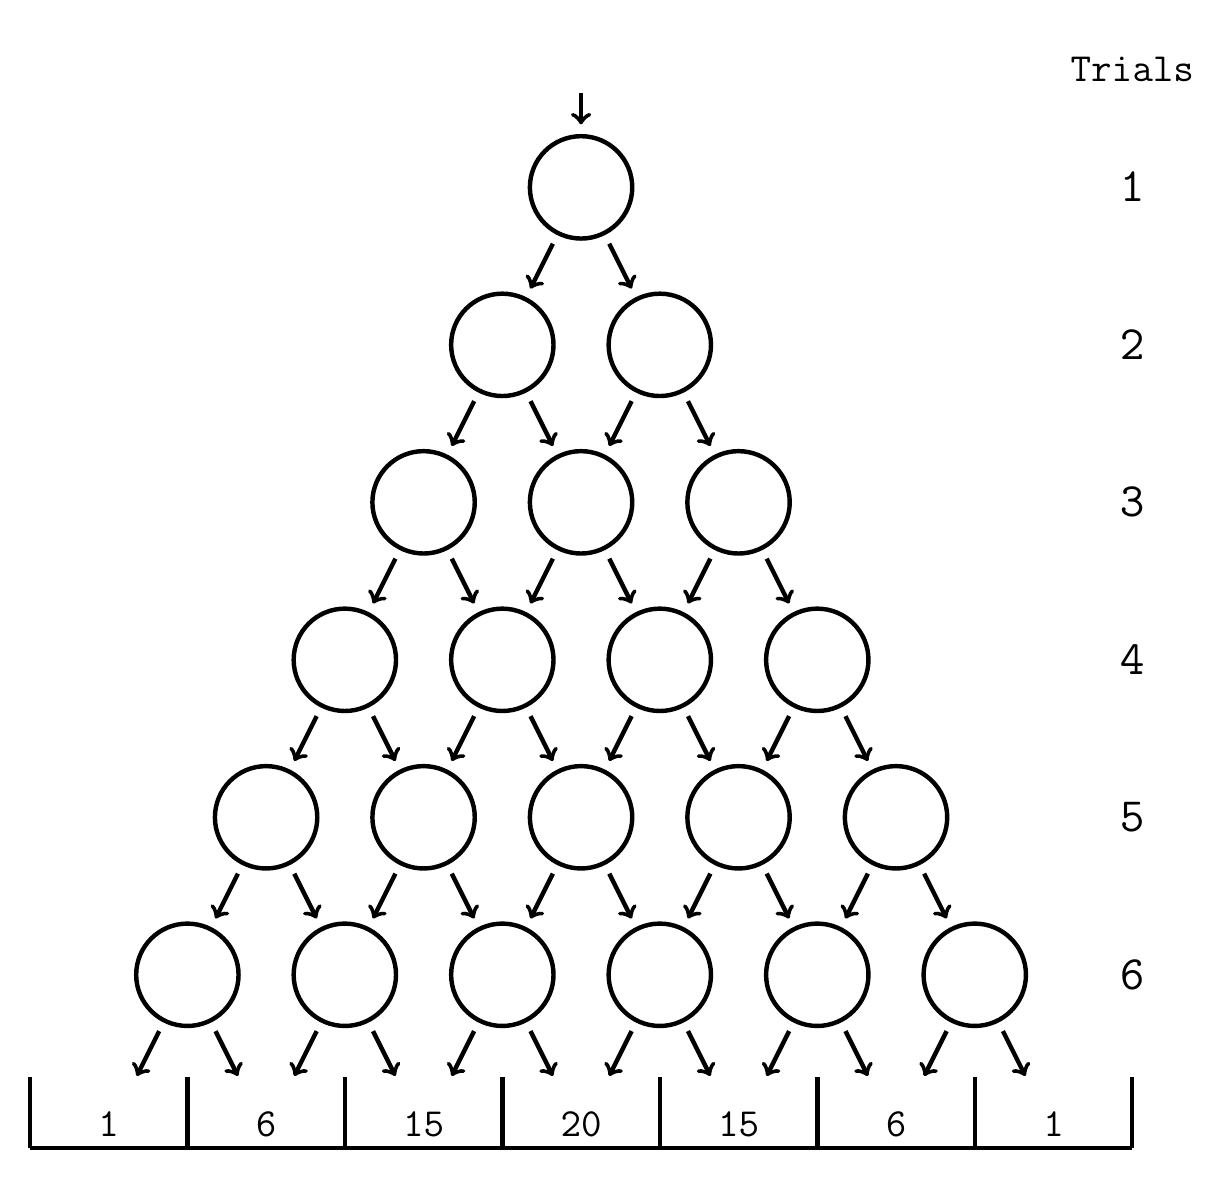
\begin{tikzpicture}[scale=.5,
      marrow/.style={->, shorten <=0.8cm, shorten >=0.8cm},
      every path/.append style={ultra thick,font=\Large\ttfamily}]
    \tikzmath{
      \Trials=6; % n_trials
      \L=4; \halfL=\L/2;
    }
    % draw balls and arrows
    \foreach \v in {1,...,\Trials} {
        \tikzmath{\y=-\L*\v;}
        \node[scale=1.2,draw=none] at (\Trials*\halfL+\L,\y) {\v};
        \foreach \i in {1,...,\v} {
          \tikzmath{\x=\i*\L-\v*\halfL;}
          \draw (\x,\y) circle [radius=1.3];
          \draw [marrow](\x,\y) -- (\x-\halfL, \y-\L);
          \draw [marrow](\x,\y) -- (\x+\halfL, \y-\L);
        }
    }

    \node at (\Trials*\halfL+\L,-1) {Trials};
    \draw [marrow] (\halfL,0) -- (\halfL,-\L);

    % draw bins and calculate frequencies for them
    \begin{scope}[yshift=-\L*\Trials*1cm-\L*1.1cm,xshift=-\L*\Trials*0.5cm]
      \foreach \i in {0,...,\Trials} {
        \draw (\i*\L,0) -- (\i*\L,.9*\halfL)
              (\i*\L+\L,0) -- (\i*\L+\L,.9*\halfL);
        \draw (\i*\L,0) -- (\i*\L+\L,0)
              node[midway, above] (TextNode) {\xintiiBinomial{\Trials}{\i}};

     }
    \end{scope}
  \end{tikzpicture}
\end{document}
